\subsection{Problems solved by AWS CloudFormation [ Author: Aqib Feroz ]}
When it is a difficult to manage and maintain the number of products and services that grow and then cloud formation has facilitated this environment, CloudFormation is the infrastructure as code tool where we can actually create a perfect clone for server setup at any time, and also manage changes in setting throughout the environment. So, let's look at the current problem with the development and delivery of multiple AWS resources in the website and ask why you can make use of cloud formation, particularly when you have to replace certain services. It is a bigger problem and with the help of Cloud Formation we can make our work easier. Currently, several challenges might arise, including considerably more time for the construction of the infrastructure and less time and less attention on the future development of the application without the cloud formation or environments without this technology. If we have to reinstall the same environment again and again, the same thing happens over and over again during a cycle construction of the infrastructure. By using CloudFormation, we can reduce this difficulty. Without CloudFormation, the bandwidth or resource required for the development of the application is not given since it takes the infrastructure to address such particular difficulties.

CloudFormation seems to be a service offering a convenient way for people to generate and control AWS resources in an organized way. This enables us to truly shape and create our AWS resources so that we can spend less time maintaining our resources and focus more on the application on which it is based.


\subsection{Introduction to AWS CloudFormation [ Author: Aqib Feroz ]}

If we manage the infrastructure we can use running scripts and books to build and manage everything, it can be a challenging version attempting to control and keeping track of the changes when it is time to multiply and test your entire production stack, but the requirement of an infrastructure stack from the script collection is not so easy. When we construct and maintain a controlled and predictable infrastructure and application stack, AWS Cloud Formation comes here.

Cloud Formation supplies and manages AWS resource based stacks and templates to construct our architecture, from a single Amazon EC2 host into a complex multi-tier, multi regional application. Cloud Formation may be used to define basic things such as Amazon VPCs and services such as AWS opsworks or AWS Beanstalk. Cloud Formation is much easier to get started, we simply create a JSON or YAML template to set the configuration of all the AWS resources in our application. Typically, Cloud Formation delivers the infrastructure and application stack as a lamp stack that can be run on Amazon EC2 and Amazon RDS.

Then we can update our CloudFormation stack any time by uploading a changed template by the AWS Management Console command line or SDK. We can also inspect our framework into the version control so that we can monitor all the modifications made with our infrastructure as well as application stack. With CloudFormation, our infrastructure architecture is controlled in a version like the software code, uploading and replicating the infrastructure into CloudFormation is easy, we can spin a replica of our production stack for the development and test with a few clicks in AWS management console. We can start ripping the mockup stacks down and rebuild whenever we really need, replication a manufacturing stack could have consumed a lot of time and could have been prone to errors if we did it manually, but with CloudFormation we can quickly and reliably create and manage AWS resource stacks.

\subsection{Features and working of CloudFormation [ Author: Aqib Feroz ]}
In this section, we will see the manner how the CloudFormation works. We have talked about the template, let’s have a deep dive in details which are features and functionality of template. Using a template, we can almost include all the application and resources that we might require, for example after the EC2 instance is provisioned and the application is already running on top of it and we want to change something in the template, so that is also possible as well. These templates are portable, if we using the template in one region we can also use the same template in the other region which will build the very similar environment in another region.

\begin{figure}[h]
    \centering
    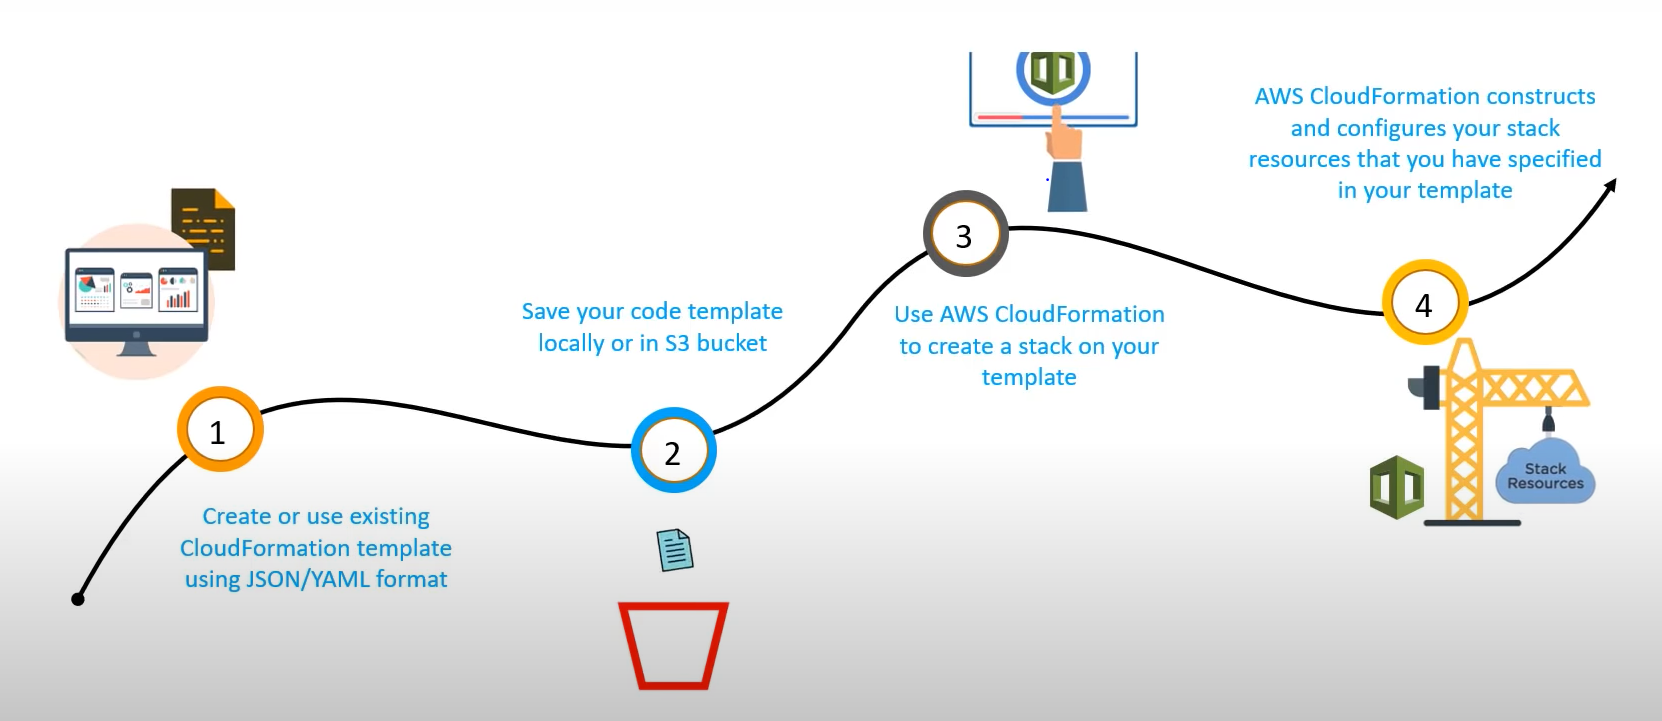
\includegraphics[scale=1.3, width=16cm, height=9cm]{images/Aqib Feroz/clfor.PNG}
    \caption{Working of CloudFormation}
    \label{fig:my_label}
\end{figure}

There are two major components in CloudFormation, Templates and Stack. These components eases the job of the administrator to manage and provision the resources. 
\subsubsection{Templates [ Author: Aqib Feroz ]}
Template in AWS CloudFormation compromises of nine main objects.

\textbf{Format version:} This defines the version number-based capabilities of the template.

\textbf{Description:} This helps us to include any arbitrary comments about what reason we are building the template.

\textbf{Metadata:} Includes the details of the resources in the template.

\textbf{Parameters:} This really helps us to customize our template. Alternatively, each time in our stack, you may enter specific values into the template.

\textbf{Mapping:} We may match a key to a collection of named values, for example to define a region based value, so we can construct a map that utilizes the name of the area as a key and then the value for each region.

\textbf{Conditions:} We may include statements that describe when creating a resource or when defining a property, such as that we may compare a value that is equivalent to another value and on the basis of this condition we can generate more resources conditionally. It is a facultative object.

\textbf{Transform:} Transform is also an optional object. This section specifies one or more transforms that we can use in our CloudFormation template. This makes template creation easier by compressing AWS infrastructure expression as code and reusing template components possible
e.g. we can condense multiple line resources declaring it into a single line in our template.


\textbf{Resources:} It states the AWS resource to be included into the stack e.g. If we want to include an EC2 instance or a S3 bucket, we would be using the resource object in our stack.

\textbf{Outputs:} Output is also optional object in template. It helps us to declare the outputs that we can import into other stacks or we can actually show it on the Cloud Formation console. E.g. we can have the output of the S3 bucket that we have already included in the template. It is easy to identify the resources that the template has provisioned in this section.

\subsubsection{Stack [ Author: Aqib Feroz ]}
Stack is a collection of AWS resource that we can mnanage in a single unit, we can create, update and delete a stack that actually means the creation, updation and deletion of resources. The stack resources are described in the Cloud Formation template and the stack can provide all necessary resources for running a web server or database server and some associated networking rules.

\textbf{Nested Stack:}
Stack could be nested as well. With Cloud Formation, we can actually nest a stack with another stack. 

\textbf{Windows Stack:}
Cloud Formation gives us the ability to construct a Windows stack based on Amazon EC2 windows, install applications and utilize a remote desktop to access and change our stack settings. These stacks may work on instances of the windows server. A range of pre- set templates are available and may be used directly from the AWS website, we have templates available for elastic beanstalk and some sample applications that runs from windows server 2008 r2.

\textbf{Stack Sets:}
Stack sets actually has taken the attack level implementation to a new level. We can build a stack set with the AWS Cloud Formation template to create the AWS account stack around the globe, using only a single template, and when the stack has been created or the stack set has been made, we can also set up, update and delete the stack in the target account and the regions. Stack sets significantly enhance the stack capability by allowing us to build, update and remove a stack over several accounts, regions and an admin account in one operation, the template may be used as the basis to provide stacks for selected target accounts throughout a given area and can be set up for the AWS Cloud Formation template management.
